\begin{frame}{The paper}
    \begin{block}{}
        \begin{itemize}
            \item Presented at ACM's SIGCOMM Conference,
            \item August 22-26, 2016,
            \item Currently cited \~{}14 times.
            \item Followed up in June of 2017.
        \end{itemize}
    \end{block}
\end{frame}

\begin{frame}{Contributions}
    \begin{block}{Contribution of the paper}
        \begin{itemize}
            \item High-level language for expressing \textcolor{ReneOrange}{network rules},
            \item \textcolor{ReneOrange}{Automatic conversion} from said rules to configuration of devices.
        \end{itemize}
    \end{block}
\end{frame}

\begin{frame}{Border Gateway Protocol (BGP) briefly}
    \begin{block}{Autonomous Systems (AS)}
        \begin{itemize}
            \item Used to connect AS's (External BGP),
            \item Can also be used within an AS (Internal BGP).
        \end{itemize}
    \end{block}
    \begin{block}{Financial Interests}
        \begin{itemize}
            \item Local policies at each AS,
            \item Desire for other to carry your traffic,
            \item Desire to avoid carrying traffic without compensation.
        \end{itemize}
    \end{block}
\end{frame}

\begin{frame}{Border Gateway Protocol (BGP) briefly (2)}
    \begin{block}{The protocol}
        \begin{itemize}
            \item Route announcements are sent to neighbors,
            \item Routes can be \textcolor{ReneOrange}{rejected} if they doesn't fit into the local policy,
            \item Neighbor AS's updates their routing information base to new routes, and announces recursively.
        \end{itemize}
    \end{block}
\end{frame}

\begin{frame}{Border Gateway Protocol (BGP) example}
    \begin{block}{Route announcement}
        \begin{itemize}
            \item AS 4 announces \code{1.2.3.4\textbackslash24}
        \end{itemize}
    \end{block}
    \begin{figure}
        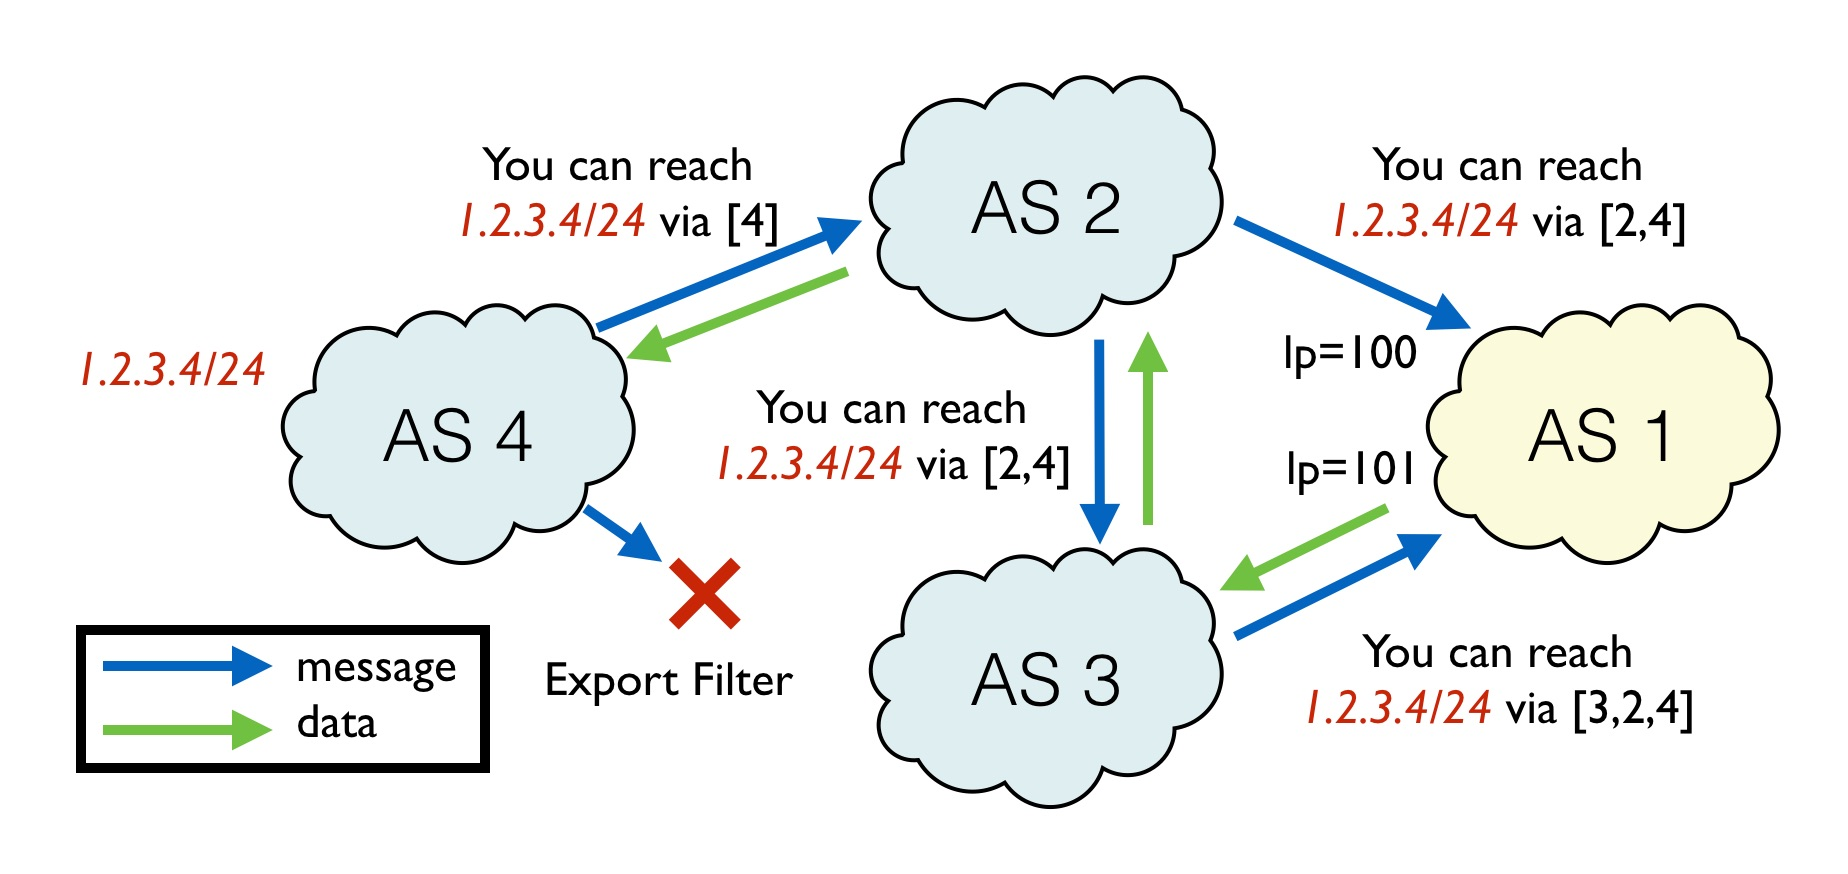
\includegraphics[height=0.45\textheight,keepaspectratio]{figures/BGP-protocol.jpg}
        \caption*{BGP example\footnote{\url{http://www.cs.princeton.edu/~rbeckett/Propane/}}}
    \end{figure}
\end{frame}

\begin{frame}{An example of policy compliance failure under link failure.}
    \begin{columns}
        \begin{column}{0.45\textwidth}
            \begin{figure}
                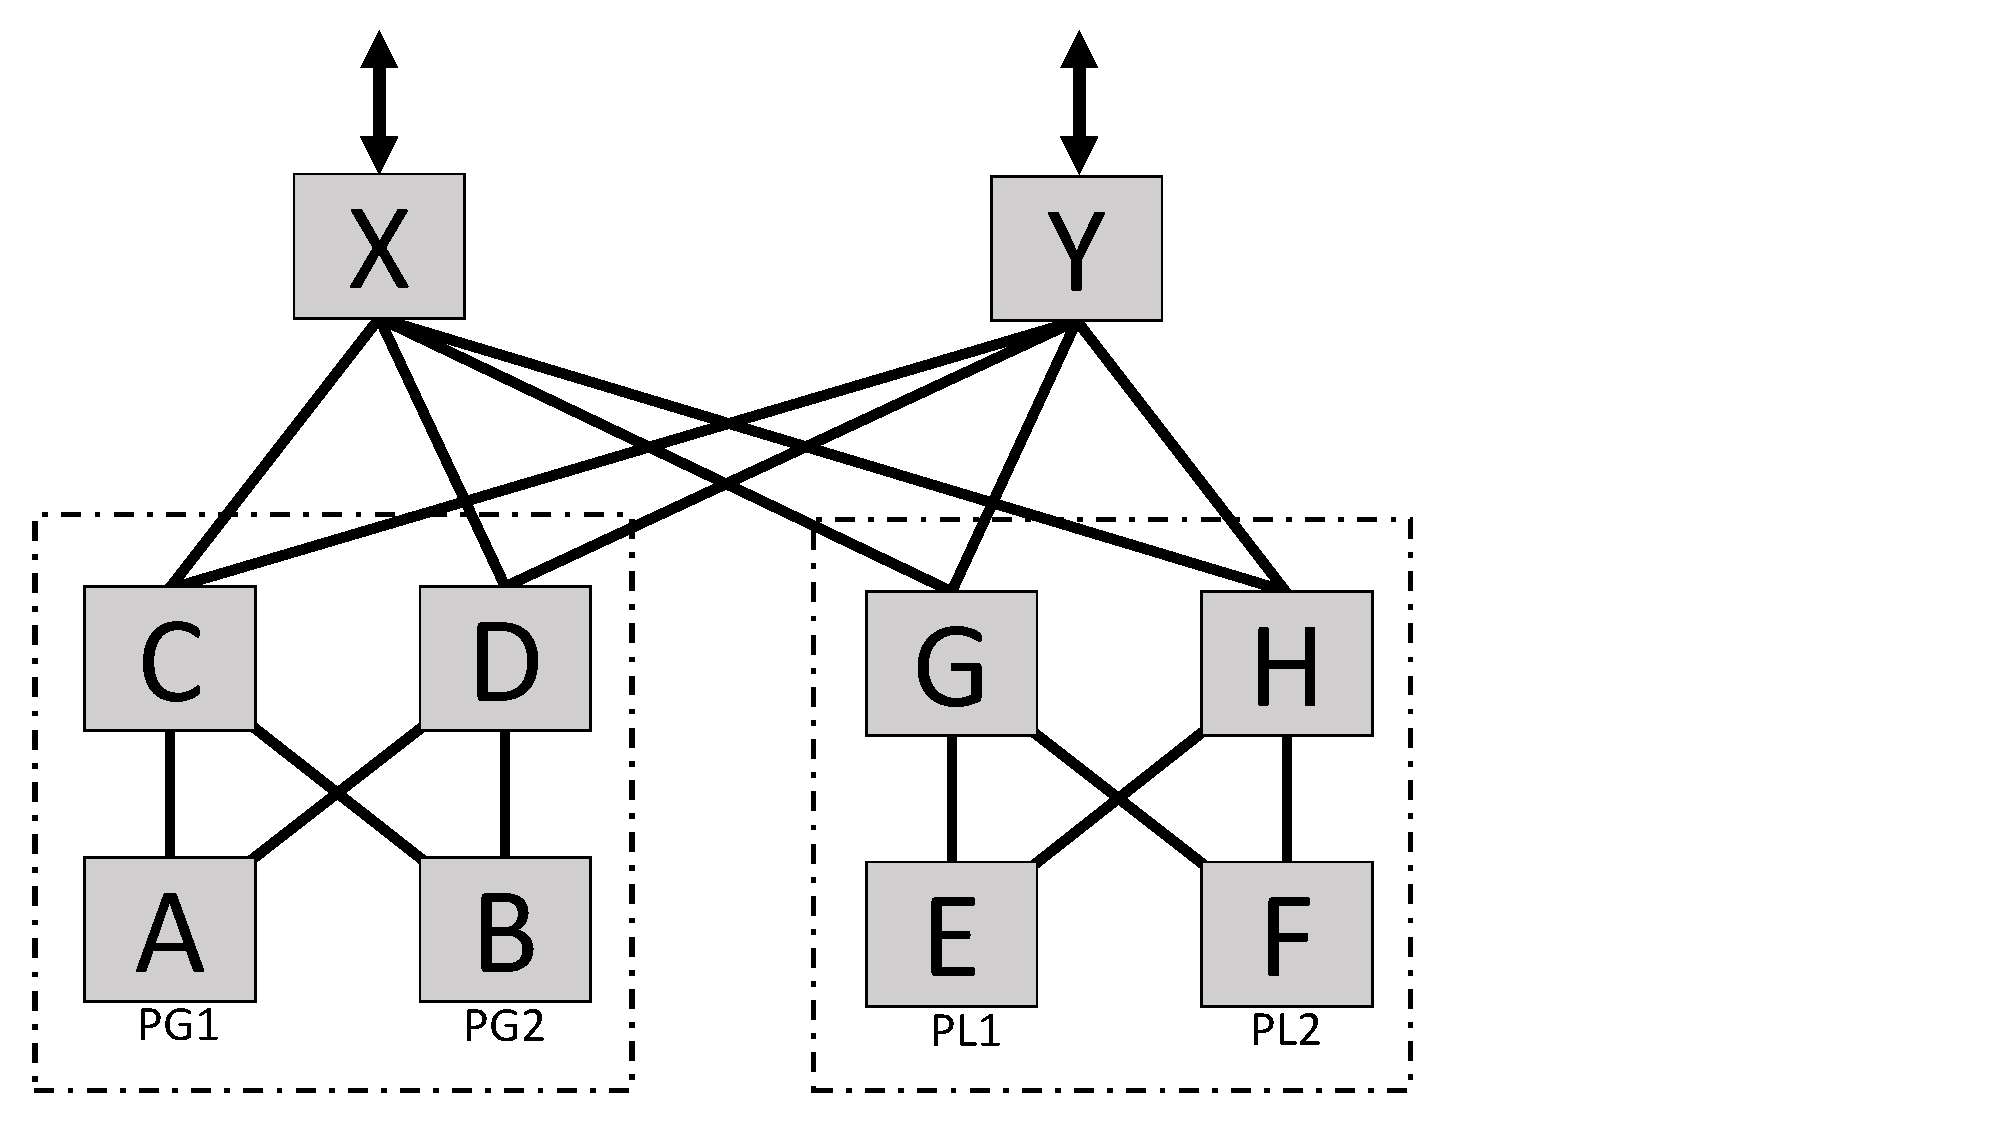
\includegraphics[width=1\textwidth,keepaspectratio,clip,trim={0cm 0cm 9cm 0cm}]{figures/ex2_clean.pdf}
            \end{figure}
        \end{column}
        \begin{column}{0.50\textwidth}
            \begin{block}{Policy}
                \begin{enumerate}
                    \item Left cluster has global services with PG* prefixes, which should be announced externally as an aggregate PG.
                    \item Right cluster has local services with PL* prefixes, which should not be announced externally.
                \end{enumerate}
            \end{block}
            \begin{block}<2>    {Policy implementation}
                \begin{enumerate}
                    \item X and Y exports routes from C and D.
                    \item X and Y doesn't export routes from G and H.
                \end{enumerate}
            \end{block}
        \end{column}
    \end{columns}
\end{frame}

\begin{frame}{An example of policy compliance failure under link failure.}
    \begin{columns}
        \begin{column}{0.45\textwidth}
            \begin{figure}
                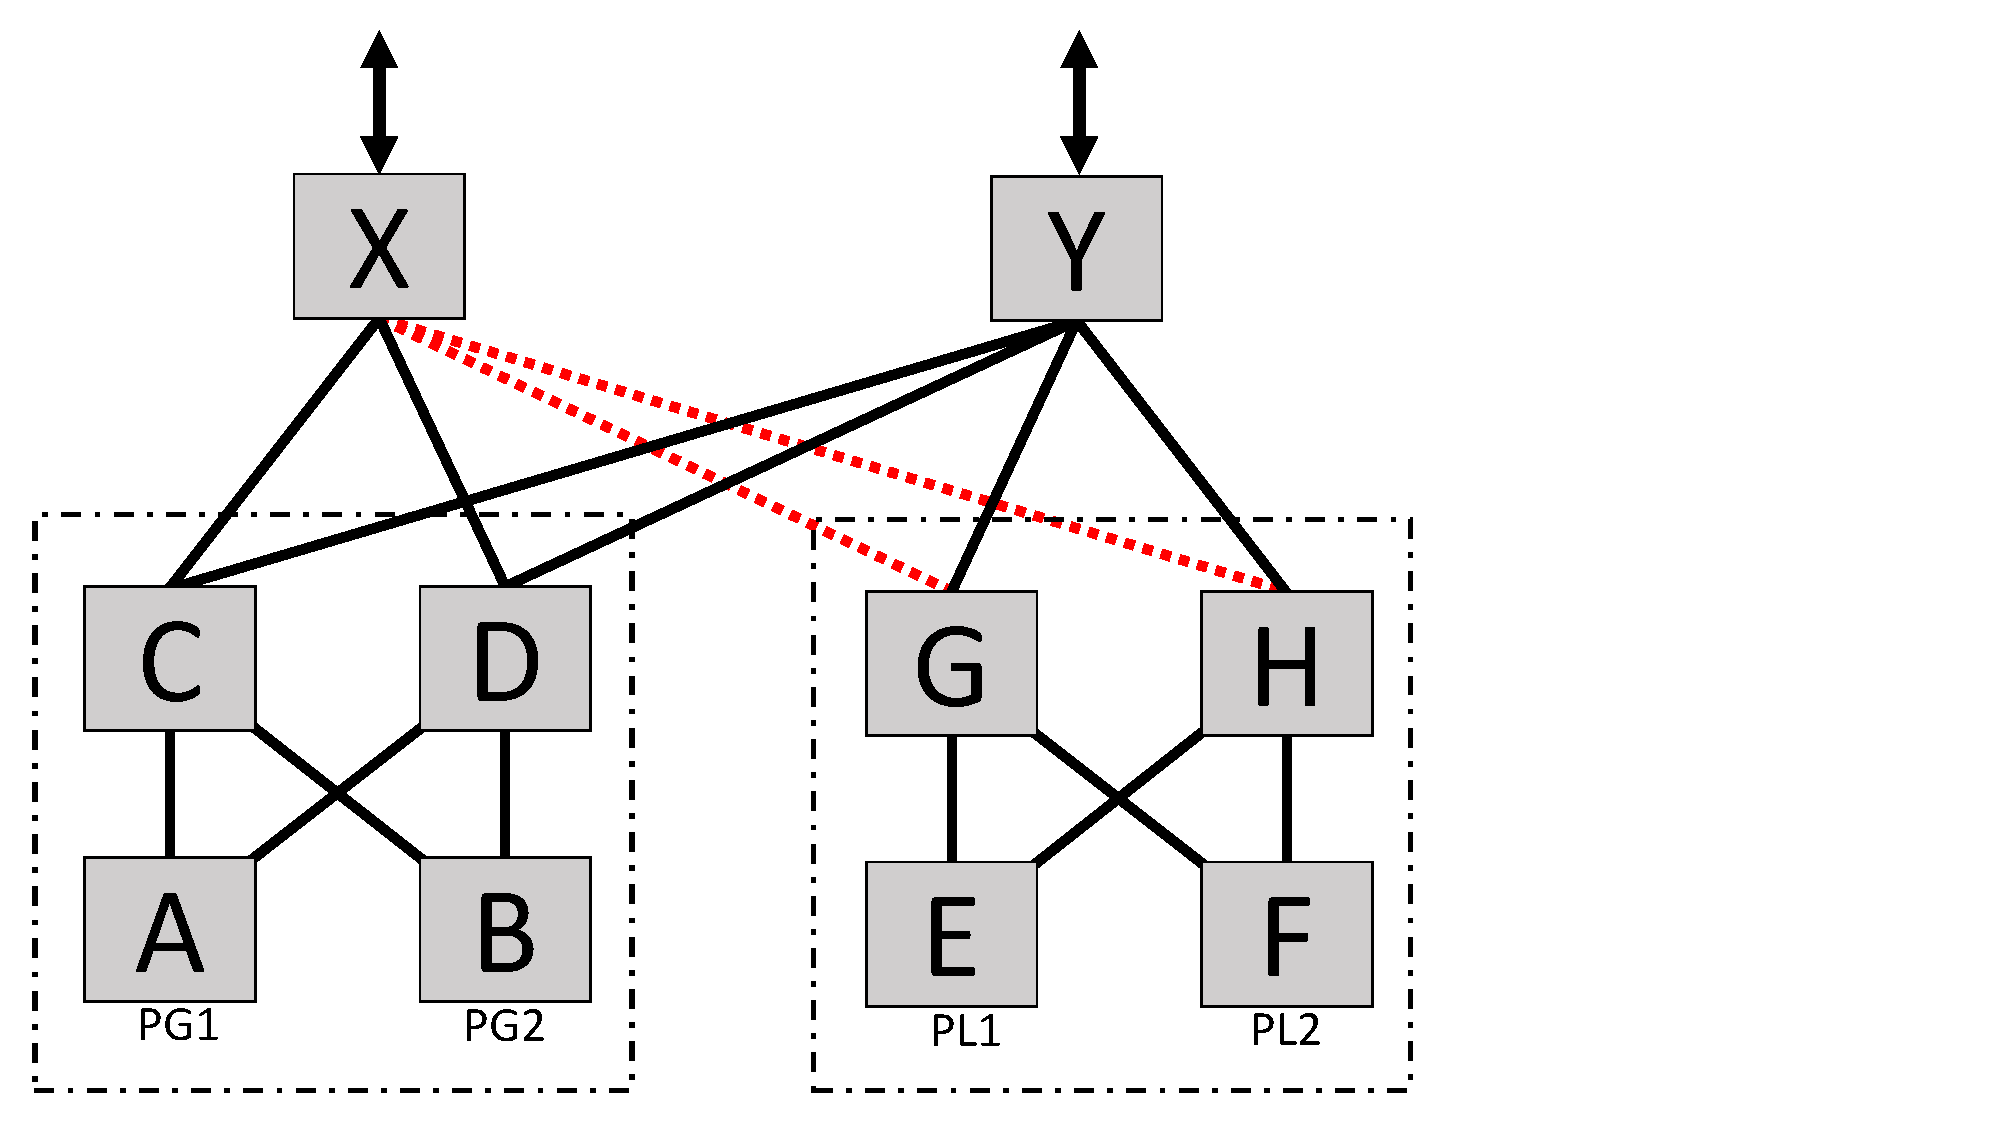
\includegraphics[width=1\textwidth,keepaspectratio,clip,trim={0cm 0cm 9cm 0cm}]{figures/ex2_1_failed_links.pdf}
                %\caption*{BGP example\footnote{\url{http://www.cs.princeton.edu/~rbeckett/Propane/}}}
            \end{figure}
        \end{column}
        \begin{column}{0.50\textwidth}
            \begin{block}{Link failures}
                \begin{itemize}
                    \item X-G
                    \item X-H
                \end{itemize}
            \end{block}
        \end{column}
    \end{columns}
\end{frame}

\begin{frame}{An example of policy compliance failure under link failure.}
    \begin{columns}
        \begin{column}{0.45\textwidth}
            \begin{figure}
                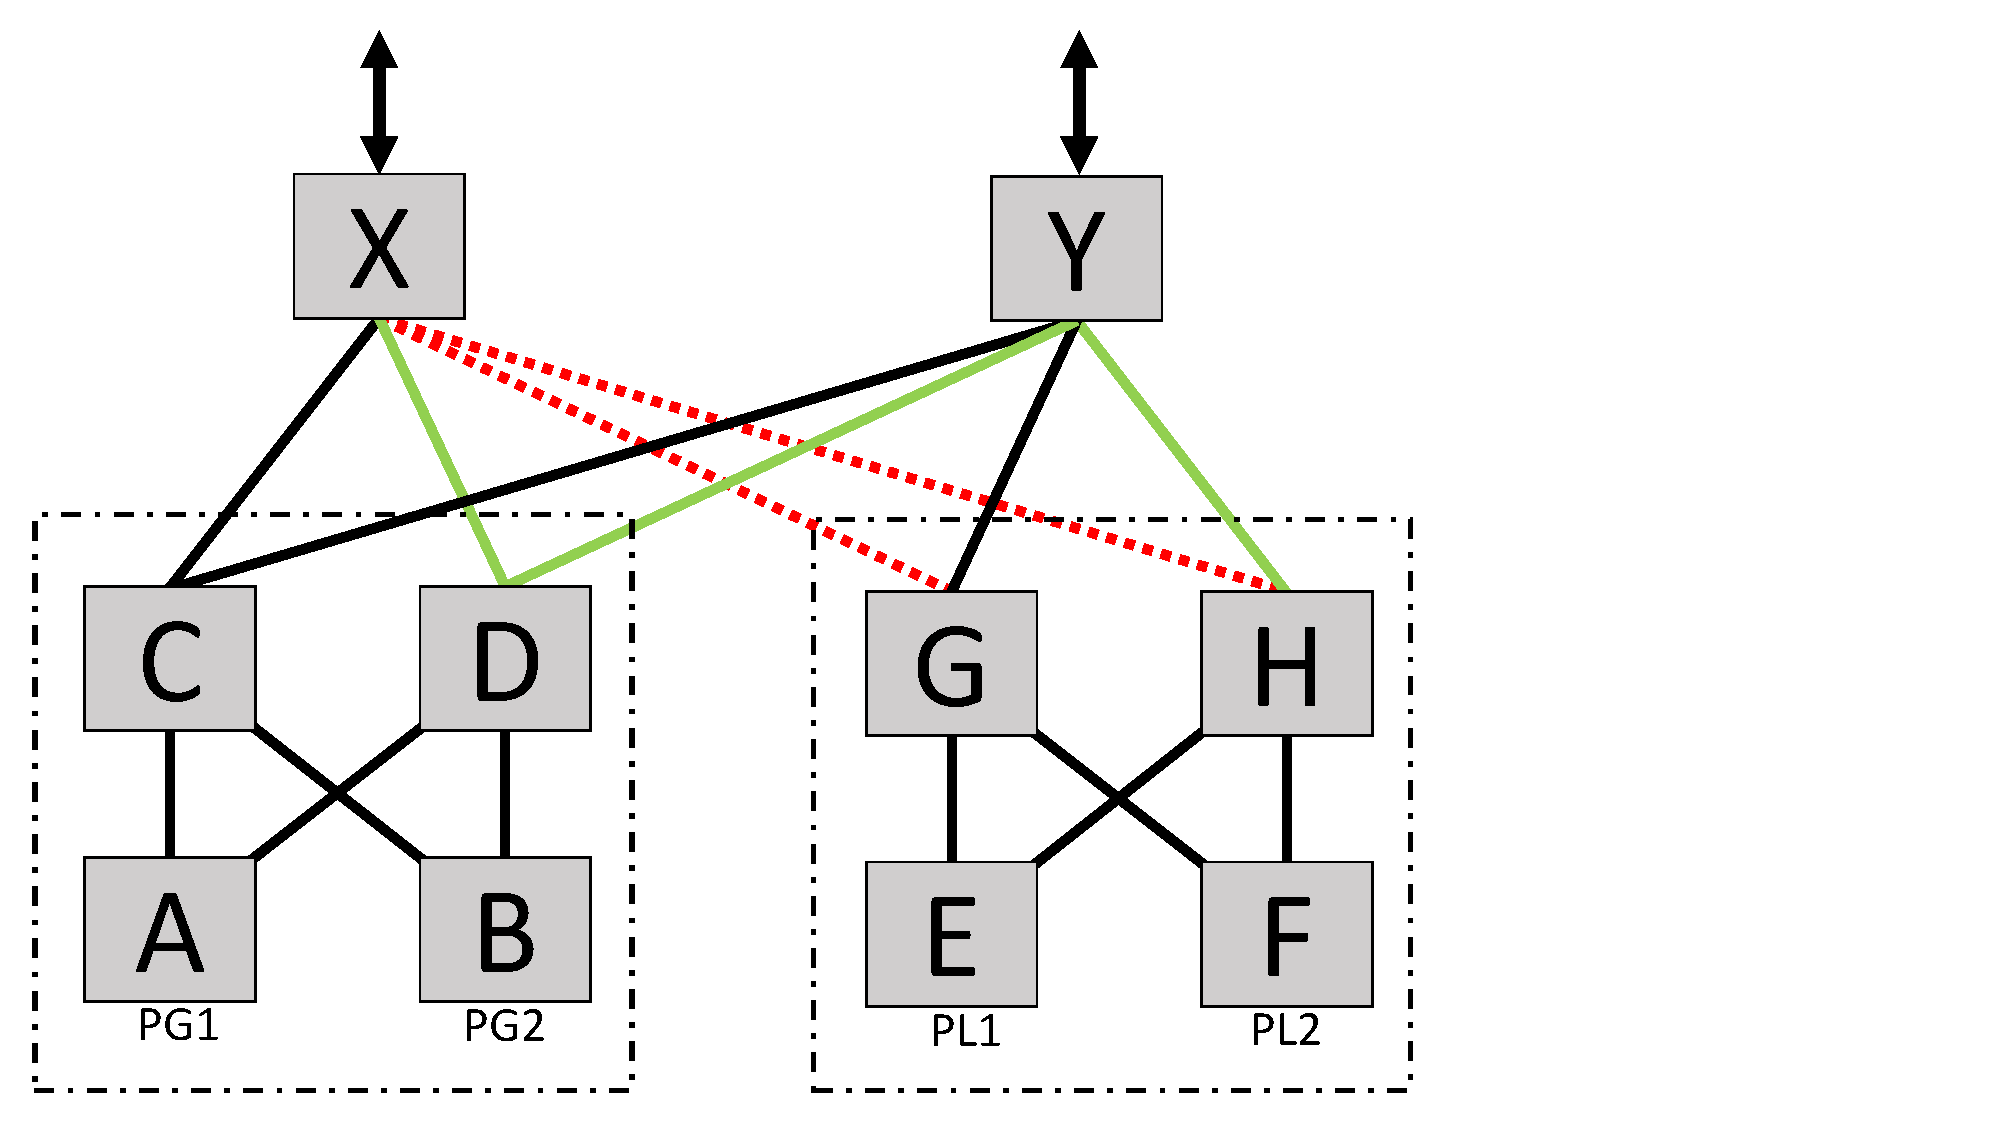
\includegraphics[width=1\textwidth,keepaspectratio,clip,trim={0cm 0cm 9cm 0cm}]{figures/ex2_1_failed_links_new_path.pdf}
                %\caption*{BGP example\footnote{\url{http://www.cs.princeton.edu/~rbeckett/Propane/}}}
            \end{figure}
        \end{column}
        \begin{column}{0.50\textwidth}
            \begin{block}{Link failures}
                \begin{itemize}
                    \item X-G
                    \item X-H
                \end{itemize}
            \end{block}
            \begin{block}{Problems}
                \begin{itemize}
                    \item H-Y-D-X
                \end{itemize}
            \end{block}
        \end{column}
    \end{columns}
\end{frame}

\begin{frame}{Bridging the Gap}
    \begin{block}{Propane}
        \begin{itemize}
            \item Compiles a network topology and a set of policies into configurations for each router.
            \item Open source\footnote{\url{https://github.com/rabeckett/propane}} compiler written in F\#.
        \end{itemize}
    \end{block}
\end{frame}

\begin{frame}{Propane overview}
    \begin{figure}
        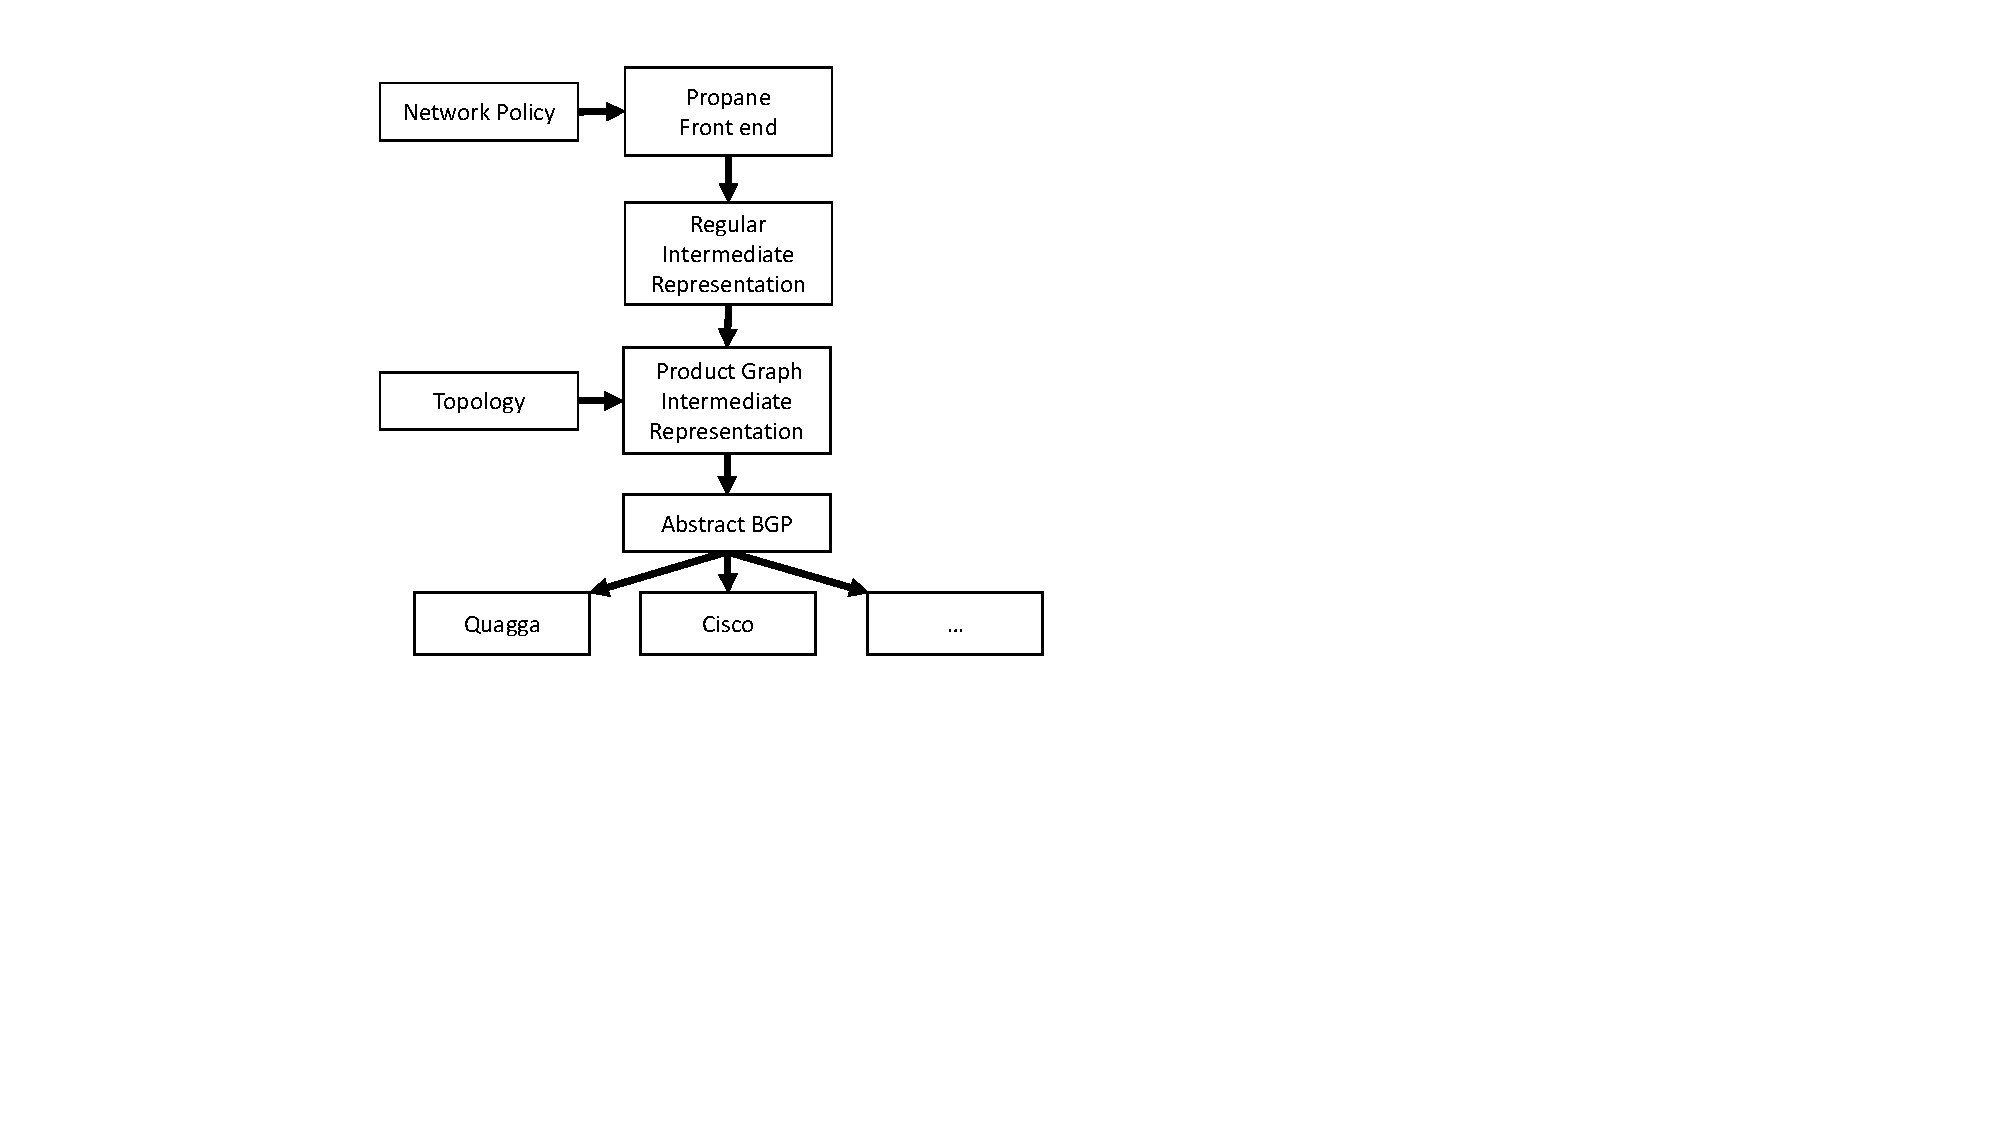
\includegraphics[height=\textheight,keepaspectratio,clip,trim={5cm 5cm 15cm 1cm}]{figures/pipeline.pdf}
        %\caption*{BGP example\footnote{\url{http://www.cs.princeton.edu/~rbeckett/Propane/}}}
    \end{figure}
\end{frame}

\begin{frame}{Product Graph Intermediate Representation (PGIR)}
    \vspace{-15pt}
    \begin{columns}
        \begin{column}{0.35\textwidth}
            Topology:\\
            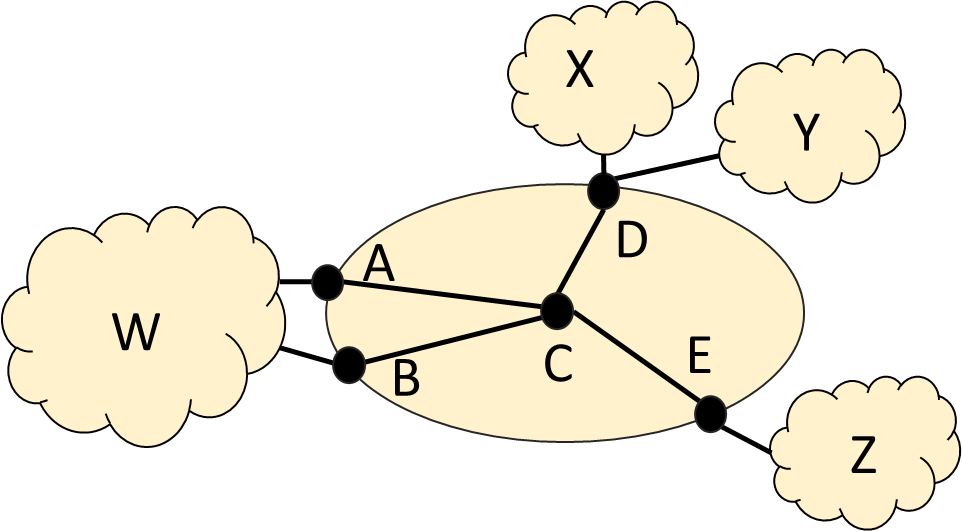
\includegraphics[width=.7\columnwidth]{figures/topology}
            \\
            Policy DFA:\\
            \resizebox{.9\columnwidth}{!}{%
                \begin{tikzpicture}[>=stealth',shorten >=1pt,auto,node distance=1.4cm,minimum size=1cm]
                    \state{0}{$0$}{              }{}
                    \state{1}{$1$}{right of=0}{}
                    \state{2}{$2$}{right of=1}{}
                    \state{3}{$3$}{right of=2}{}
                    \state{4}{$4$}{right of=3}{}
                    \state{5}{$5$}{right of=4}{accepting}
                    \transition{0}{1}{out}{}
                    \transition{1}{2}{D}{}
                    \transition{2}{3}{C}{}
                    \transition{3}{4}{A}{}
                    \transition{4}{5}{W}{}
                \end{tikzpicture}
            }
            \resizebox{.9\columnwidth}{!}{%
                \begin{tikzpicture}[>=stealth',shorten >=1pt,auto,node distance=1.6cm]
                    \state{0}{$0$}{              }{}
                    \state{1}{$1$}{right of=0}{}
                    \state{2}{$2$}{right of=1}{}
                    \state{3}{$3$}{right of=2}{}
                    \state{4}{$4$}{right of=3}{accepting}
                    \transition{0}{1}{out}{}
                    \transition{1}{2}{in}{}
                    \transition{2}{2}{A,C,D,E}{loop above}
                    \transition{2}{3}{B}{}
                    \transition{3}{3}{B}{loop above}
                    \transition{3}{2}{A,C,D,E}{bend left}
                    \transition{3}{4}{W}{}
                \end{tikzpicture}
            }
        \end{column}
        \begin{column}{0.01\textwidth}
             $\Rightarrow$
        \end{column}
        \begin{column}{0.45\textwidth}
            \begin{figure}[htb]
                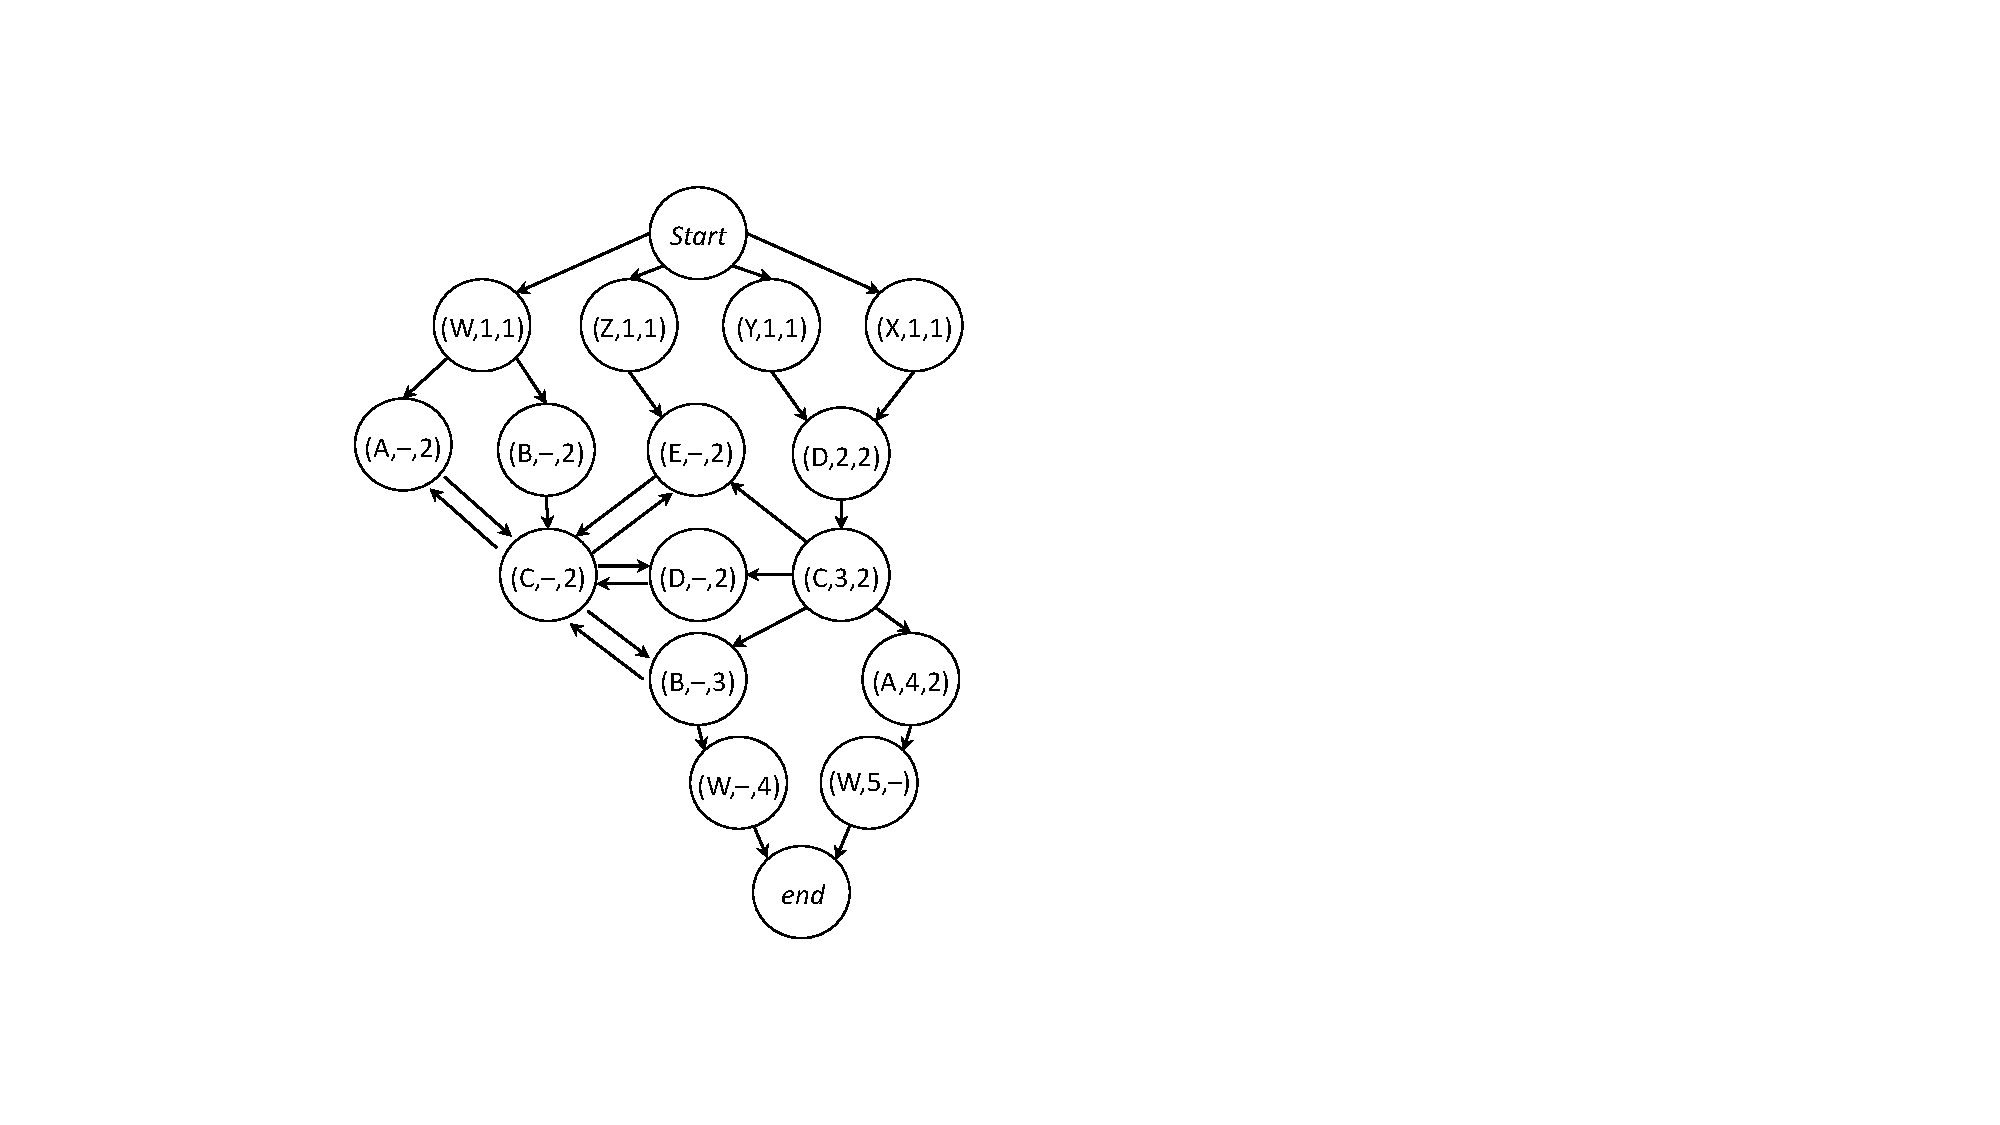
\includegraphics[height=\textheight,keepaspectratio,clip,trim={5cm 0cm 16cm 2cm}]{figures/pgir.pdf}
            \end{figure}
        \end{column}
    \end{columns}
\end{frame}

\begin{frame}{Analyzing the PGIR}
    \begin{block}{Failure-safety}
        \begin{itemize}
            \item Regret-free preferences
            \item Avoiding loops
        \end{itemize}
    \end{block}
    \begin{block}<2>{Aggregation-safety}
        \begin{itemize}
            \item Avoid black hole traffic for up to \textit{k} failures.
            \item Can be seen as a variation of the min-cut problem.
        \end{itemize}
    \end{block}
\end{frame}

\begin{frame}{Results using Propane}
    \begin{columns}
        \begin{column}{0.45\textwidth}
            \begin{figure}
                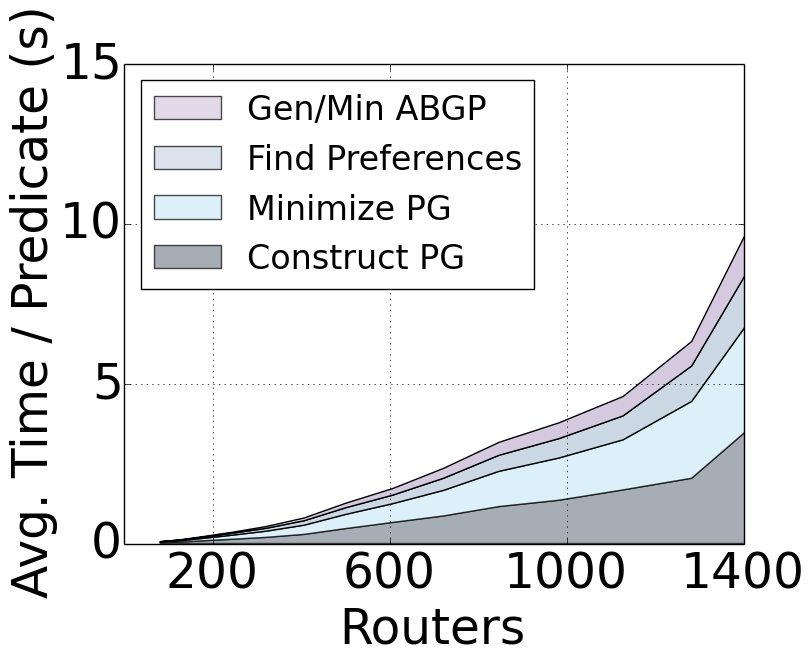
\includegraphics[width=0.66\columnwidth,keepaspectratio]{figures/compilation-times-dc}
            \end{figure}
        \end{column}
        \begin{column}{0.50\textwidth}
            \begin{block}{Expressiveness}
                \begin{itemize}
                    \item Not tested, only from informal interviews,
                    \item Network operators verified semantic preservation,
                    \item Could translate all network policies.
                \end{itemize}
            \end{block}
            \begin{block}{Propane vs. Operator written configurations}
                \begin{itemize}
                    \item Sometimes utilizing different BGP mechanisms for the same result.
                \end{itemize}
            \end{block}
        \end{column}
    \end{columns}
\end{frame}

\begin{frame}{Conclusion}
    \begin{block}{Propane}
        \begin{itemize}
            \item Takes in the topology and a high level policy of a network,
            \item Generates a configuration for each router in the network.
            \item Correct by construction.
        \end{itemize}
    \end{block}
\end{frame}
